\chapter{joint and conditional distributions}
\section{random vector and joint distributions}
\subsection{random vector}
\begin{definition}{random vector}
对于 prob space $(\Omega, \mathcal{F}, P)$, 
一个 function $\mathbf{X}: \Omega \to \mathbb{R}^n$ 如果是一个
$(\mathcal{F}, \mathcal{B}(\mathbb{R}^n))$-measurable function, 则
称它为一个 $n$-dimensional random variable, 或者 $n$-dimensional random vector.

通常我们将 random vector 写成分量形式
$$\mathbf{X}(\omega) = (X_1(\omega), X_2(\omega), \dots, X_n(\omega))^T$$
\end{definition}
random vector 相当于在一个 prob space 上, 考虑多个重新分配 mass 的方法, 并把它们并列起来.
\begin{proposition}{由 \(n\) 个 random variable 构成的 vector 是一个 random vector}
    令 \(X_1, X_2, \cdots, X_n\) 
    是定义在\textbf{同一个 prob space} \((\Omega, \mathcal{F}, \bP)\) 
    上的 \(n\) 个 random variables. 则函数 \(\mathbf{X}: \Omega \to \bR^n\) defined by 
    \[
    \omega \mapsto (X_1(\omega), X_2(\omega), \cdots, X_n(\omega))^T
    \]
    是一个 random vector.
\end{proposition}
\begin{proof}
    我们在 measure theory 中证明过: 对于任意的 finite seq of Borel measureable functions 
    \( (  {f_i}: \Omega \to \mathbb{R} )_{i=1}^k\), 其各作为一个维度组成的函数
    \(f = (f_1,\cdots, f_k)\) 也是一个 Borel measurable function (from \(\Omega\) 到 \(\mathbb{R}^k\)).
\end{proof}
\begin{proposition}{一个 random vector 的每个分量都是一个 random variable}
    令 \(\mathbf{X} = (X_1, X_2, \cdots, X_n)^T\) 是一个 random vector. 
    则对于任意 \(i\), \(X_i\) 都是一个 random variable.
\end{proposition}
\begin{proof}
    对于 $\mathbf{X}: \Omega \to \mathbb{R}^n$ 是 $(\mathcal{F}, \mathcal{B}(\mathbb{R}^n))$-measurable,
    我们可以将第 $i$ 个分量 $X_i$ 看作是 composition of two maps: 
    $$X_i = \pi_i \circ \mathbf{X}$$
    其中 $\pi_i: \mathbb{R}^n \to \mathbb{R}$ projection map  $\pi_i(x_1, \dots, x_n) = x_i$.\\
    由于 projection map $\pi_i$ 是一个 Borel measurable function, 我们可以得出: \(X_i = \pi_i(\mathbf{X})\) 也是
一个 Borel measurable function, 也就是一个 random variable.
\end{proof}

\begin{remark}
上两条 propositions 说明了一个事情: random vectors 和其分量 random variables 完全相互决定.
\begin{itemize}
    \item\textbf{ random variables 组合起来一定是一个 random vector.}
    \item \textbf{random vector 拆开每个分量一定是 random variable.}
\end{itemize}
因而, 研究一个 random vector 也就相当于研究分量 random variables 之间的关系. 

这一章节我们会从 random vector 的性质 
(比如 \textbf{joint distribution 和 marginal distribution, conditional distribution}) 
出发, 研究分量 random variables 之间的关系.

(但是注意: 前提是这些 random variables 必须定义在同一个 prob space 上. 也就是, 它们的 base 
probability measure 一定相同. 如果我们考虑不同 prob space 上的 random variables 的话, 
那它们没有一个公共的 base probability measure, 很难说它们之间有什么关系. 
这种情况下, 我们需要 coupling: 构造一个新的 prob space (说白了就是 product space),
让这两个 random variables 都有一个新 version. 这一问题我们之后再讨论.)
\end{remark}

\subsection{joint distribution}
\begin{definition}{joint distribution and joint cdf}
    令 \(X_1,\cdots, X_n\) 为 RV from the same prob space. 
    即 \(\mathbf{X}:= (X_1,\cdots, X_n)\) 
    是一个 random vector.

    我们称 \(\bP^{\mathbf{X}}: \bR^n \to \bR\) defined by 
    $$\bP^{\mathbf{X}}(B) = \bP(\mathbf{X}^{-1}(B)), \quad \forall B \in \mathcal{B}(\mathbb{R}^n)$$
    为 \(X_1, \cdots, X_n\) 的 \textbf{joint distribution}.
    
    而我们称 \(F_{\mathbf{X}} = F_{X_1,
    \cdots, X_n}: 
    \bR^n \to \bR\) defined by   
     \[
    F_{\mathbf{X}}(x_1,\cdots,x_n) = \bP(X_1 \leq x_1, \cdots, X_n \leq x_n)
    \]
     (即 \(\bP^{\mathbf{X}}\) restricted to the set of rectangles
     \(\{(-\infty, x_1] \times \cdots \times (-\infty, x_n]: (x_1,\cdots,x_n) \in \bR^n\}\))
    为它们的 \textbf{joint distribution function (或称 joint cdf)}.
\end{definition}
joint distribution 的定义已经包括了如何从多个 random variables 的 distributions
得到一个 joint distribution.
而, 我们也可以从一个 joint distribution 的 limit behavior 
得到每个 random variable 分量的 distributions, 称之为 marginal distribution:
\begin{definition}{marginal distribution}
    令 \(\mathbf{X} = (X_1, \cdots, X_n)^T\) 是一个 random vector. 
    则对于任意 \(i\), \(X_i\) 的 distribution \(\bP^{X_i}\) 
    被称为 \(\mathbf{X}\) 的第 \(i\) 个分量的 \textbf{marginal distribution}.
\end{definition}
我们以 \(\bR^2\) 为例. 得出的结论可以推广到 \(\bR^n\).
\begin{proposition}{通过 joint distribution 的 limit behavior 得到 marginal distribution}
    令 \(\mathbf{X} = (X_1, X_2)^T\) 是一个 random vector. 
    则对于任意 \(x\in \bR\), 有
    \[\bP(X_1 \leq x) = \lim_{y\to \infty} F_{\mathbf{X}}(x,y)\]
    \(X_2\) 的 marginal distribution 也可以通过同样的方法得到.

    此外, joint distribution 有其他明显的 limit behaviors:
    \begin{itemize}
        \item \[ \lim_{x\to -\infty}F(x,y) = \lim_{y\to -\infty}F(x,y) = 0 \]
        \item \(F_{\mathbf{X}}\) 对于每个维度都是 increasing 且 right-continuous 的.
        \item \[ \bP(X\leq x, Y \leq y) = \lim_{z\uparrow y} F(x,z) = \lim_{z\uparrow x} F(z,y) = \lim_{z_1\uparrow x, z_2 \uparrow y}F(z_1, z_2) \]
        \item \[ \bP(x_1 \leq X \leq x_2, y_1 \leq Y \leq y_2) = F(x_2,y_2) - F(x_1,y_2) = F(x_2,y_1)+F(x_1,y_1) \]
    \end{itemize}
\end{proposition}
\begin{remark}
    最后一条: 右边相当于 
    \[
    \bP(x_1 < X < x_2, Y < y_2) - \bP(x_1 < X < x_2, Y < y_1) 
    \]
    因而成立.
\end{remark}

discrete random vector 很容易处理. 我们可以直接定义 joint pmf.
而 continuous random vector 需要展开讨论. 接下来我们讲单独讨论
continuous random vector 的 joint distribution.

\subsection{condinuous joint cdf 与 joint pdf}
recall:
 一个随机变量 \(X\) 被称为一个 continuous random variable, 如果它的
cdf 是 absolutely continuous 的. 这个条件也等价于, 存在一个函数 \(f_X: \bR \to [0,\infty)\) 
使得 \[
F_X(x) = \int_{-\infty}^x f_X(t) \, dt
\]

这个定义可以 generalize 到 random vector 上.
\begin{definition}{continuous random vector 和 continuous joint cdf}
    对于 random vector  \(\mathbf{X} = (X_1,\cdots, X_n)^T\) 
    如果 \(\bP^{\mathbf{X}} \ll \lambda^n\),
    即存在一个函数 \(f_{\mathbf{X}}: \bR^n \to [0,\infty)\) 使得对于任意 Borel set \(B \subseteq \bR^n\), 有
\[\bP^{\mathbf{X}}(B) = \int_B f_{\mathbf{X}}(x_1, \cdots, x_n) \, d\lambda^n(x_1, \cdots, x_n)\]
    则称 \(\mathbf{X}\) 是一个 \textbf{continuous random vector}.

    注意: 由于是在 \(\bR^n\) 上, 这等价于存在一个函数 \(f_{\mathbf{X}}: \bR^n \to [0,\infty)\) 使得对于任意 \(x_1, \cdots, x_n\), 有
     \[F_{\mathbf{X}}(x_1, \cdots, x_n) = \int_{-\infty}^{x_1} \cdots \int_{-\infty}^{x_n} f_{\mathbf{X}}(t_1, \cdots, t_n) \, dt_n \cdots dt_1\]
\end{definition}
\begin{remark}
    这个函数 \(f_{\mathbf{X}}\) 
    就是 continuous random vector \(\mathbf{X}\) 
    的 \textbf{joint probability density function (joint pdf).}
    它是 joint distribution measure \(\bP^{\mathbf{X}}\) 
    对于 Lebesgue measure \(\lambda^n\) 的 Radon-Nikodym derivative: \[\frac{d\bP^{\mathbf{X}}}{d\lambda^n} = f_{\mathbf{X}}\]
\end{remark}
\begin{remark}
    我们已经知道, 只要存在导数 \(f_{\mathbf{X}}\) 可以对于任意 \(\mathbf{x}\in \bR^n\) 
    还原出 joint cdf \(F_{\mathbf{X}}\) 的值, 那么 \(f_{\mathbf{X}}\) 就是 joint pdf, 
    这个 random vector 就是一个 continuous random vector.

    那么这个还原积分的计算可以任意换序吗? 

    显然是可以的. 因为 recall \textbf{Fubini's theorem}: 只要 \(f\) 绝对可积, 即 
    \(\int_{\bR^n} |f| \, d\lambda^n < \infty\), 
    那么对于任意的 permutation \(\sigma\) of \(\{1,2,\cdots,n\}\), 我们都可以将积分的顺序换成
     \[\int_{-\infty}^{x_{\sigma(1)}} \cdots \int_{-\infty}^{x_{\sigma(n)}} 
     f(t_1, \cdots, t_n) \, dt_{\sigma(n)} \cdots dt_{\sigma(1)}\]
    而我们知道, \(f\) 一定是非负的, 而且积分一定是 1, 因而可以任意换序积分. 
    
    这就很舒服. 这也给出了 margin distribution 的计算方法: 
    只要对 joint pdf \(f_{\mathbf{X}}\) 在其他维度上积分掉就行了.
\end{remark}
\begin{remark}
    注意: \textbf{多个 continuous random variables 的 joint distribution 
    不一定是 continuous 的.}
    反例: 考虑 random vector \(\mathbf{X} = (X, X)^T\) where \(X \sim \text{Uniform}(0,1)\)
    则 $\bP((X,X) \in \{y=x\}) = 1$. 而注意, \(\{y=x\}\) 在 \(\bR^2\) 中的 Lebesgue measure 为 0, 
    而 absolute continuity 要求: 对于一个零测集, 其 \(\bP^{\mathbf{X}}\) 测度也必须是 0 (这是 \(\bP^{\mathbf{X}} \ll \lambda^n\) 的标准定义), 
    因而 joint distribution 不是 continuous 的.
\end{remark}

\begin{proposition}{joint pdf 和 joint cdf 的性质}
令 \(\mathbf{X} = (X_1, \cdots, X_n)^T\) 是一个 continuous random vector, 
则它的 joint pdf \(f_{\mathbf{X}}\) 和 joint cdf \(F_{\mathbf{X}}\) 有以下性质: 
    \begin{itemize}
        \item \(f_{\mathbf{X}}\geq 0\) a.e. 并且 \(\int_{\bR^n} f_{\mathbf{X}} \, d\lambda^n = 1\).
\item (如果一个集合 \(A\) 有一个零测维度, 那么 \(\bP^{\mathbf{X}}(A) = 0\))
\[\bP(X_1 = x_1
, x_2 \leq X_2 \leq x'_2  \cdots,  x_n \leq  X_n \leq x'_n) = 0\]

\item 每个 \(X_i\) 的 marginal distribution 也是 (absolutely) continuous 的,
并且 \[
f_{X_i}(x) = \int_{\bR^{n-1}} f_{\mathbf{X}}(t_1, \cdots, t_{i-1}, x, t_{i+1}, \cdots, t_n) \, dt_1 \cdots dt_{i-1} dt_{i+1} \cdots dt_n
\]
例如, \[
f_{X}(x) = \int_{-\infty}^\infty f_{\mathbf{X}}(x,y) \, dy
\]
\item 对每个 \(x_1, \cdots, x_n \in \bR\), 都可以通过偏导数从 joint cdf 得到 
joint pdf (这个偏导数一定 (a.e.) 存在):
\[
f_{\bf{X}}(x_1,\cdots,x_n) = \frac{\partial^n}{\partial x_1 \cdots \partial x_n} F_{\mathbf{X}}(x_1, \cdots, x_n)
\]
并且 by Fubini's theorem 可以 (a.e.) 任意换序:
$$\frac{\partial^n}{\partial x_{\sigma(1)} \dots \partial x_{\sigma(n)}} F_{\mathbf{X}} \stackrel{a.e.}{=} f_{\mathbf{X}}$$
\end{itemize}
\end{proposition}
\begin{proof}

\begin{itemize}
    \item 由于 \(f_{\mathbf{X}}\) 是 \(\bP^{\mathbf{X}}\) 对于 \(\lambda^n\) 的 Radon-Nikodym derivative, 
    因为任何 Borel 集 $B$ 都有 $P^{\mathbf{X}}(B) \ge 0$,
     假设存在一个集合 $A \in \mathcal{B}(\mathbb{R}^n)$ 
     使得在其上 $f_{\mathbf{X}} < 0$ 且 $\lambda^n(A) > 0$, 
    那么根据积分定义$$\bP^{\mathbf{X}}(A) = \int_A f_{\mathbf{X}} \, d\lambda^n < 0$$
    因而反证得 \(f_{\mathbf{X}} \geq 0\) a.e. 

    并且 \[\int_{\bR^n} f_{\mathbf{X}} \, d\lambda^n = \bP^{\mathbf{X}}(\bR^n) = 1\]

\item natural.
\item 即 marginal distribution 的定义在 continuous case 中的展开
\item by Fubini's theorem, 以及 joint cdf 的定义.
\end{itemize}
    \end{proof}

\begin{example}
考虑 
\[
f_{X, Y}(x, y)= \begin{cases}c e^{-x} e^{-2 y}, & \text { if } x, y>0 \\ 0, & \text { otherwise }\end{cases}
\]
Find \(c\) 使得这是一个合法的 joint pdf, 
并且计算 \(X\) 和 \(Y\) 的 marginal pdfs, 以及 \(\bP(X>1, Y<1)\).
\begin{solution}
我们需要
$$c \left( \int_{0}^{\infty} e^{-x} dx \right) \left( \int_{0}^{\infty} e^{-2 y} dy \right) = 1$$
evaluate 这两个积分:
$$\int_{0}^{\infty} e^{-x} dx = \left[ -e^{-x} \right]_{0}^{\infty} = 1,$$
$$\int_{0}^{\infty} e^{-2 y} dy = \left[ -\frac{1}{2} e^{-2 y} \right]_{0}^{\infty} = \frac{1}{2}$$
因为 \(c\) 必须为 2.

计算 \(X\) 的 marginal pdf:
$$f_X(x) = \int_{0}^{\infty} 2 e^{-x} e^{-2 y} dy = 2 e^{-x} \left[ -\frac{1}{2} e^{-2 y} \right]_{0}^{\infty} = e^{-x}$$
然后计算 \(Y\) 的 marginal pdf:
$$f_Y(y) = \int_{0}^{\infty} 2 e^{-x} e^{-2 y} dx = 2 e^{-2 y} \left[ -e^{-x} \right]_{0}^{\infty} = 2 e^{-2 y}$$
最后计算 \(\bP(X>1, Y<1)\):
$$\bP(X > 1, Y < 1) = \int_{1}^{\infty} \int_{0}^{1} 2 e^{-x} e^{-2 y} dy dx = \left( \int_{1}^{\infty} e^{-x} dx \right) \left( \int_{0}^{1} 2 e^{-2 y} dy \right)$$
这两个定积分分别为:
$$\int_{1}^{\infty} e^{-x} dx = \left[ -e^{-x} \right]_{1}^{\infty} = e^{-1},$$
$$\int_{0}^{1} 2 e^{-2 y} dy = \left[ -e^{-2 y} \right]_{0}^{1} = 1 - e^{-2}$$ 
因而$$\bP(X > 1, Y < 1) = e^{-1} (1 - e^{-2}) = e^{-1} - e^{-3}$$
\end{solution}
\end{example}

\begin{theorem}
    对于 continuous random vector \(\mathbf{X} = (X_1, \cdots, X_n)^T\),
取任意 Borel measurable function \(g: \bR^n \to \bR\),
则 \(g(\mathbf{X})\) 是一个 random variable, 并且如果 \(\bE[|g(\mathbf{X})|] < \infty\), 则
, 则
$$\bE[g(\mathbf{X})] = \int_{\bR^n} g(\mathbf{x}) f_{\mathbf{X}}(\mathbf{x}) \, d\lambda^n(\mathbf{x})$$
\end{theorem}

\begin{example}
    Let $(X, Y)$ be a two-dimensional random variable with joint density function
     $$ f_{X, Y}(x, y)= \begin{cases}1, & 0<\frac{y}{2}<x<1 \\ 0, & \text { otherwise }\end{cases} $$ 
\begin{itemize}
    \item [(a)] 求 marginal density $f_Y$
    \item [(b)] 计算概率 $\mathbb{P}(X=1 / 2)$ 和 $\mathbb{P}(X+Y \leq 3 / 2)$
\end{itemize}
\begin{solution}
\begin{itemize}
\item [(a)] 
对固定 $y$ 需要满足 $0<y<2 x$ 且 $x<1$, 等价于 $x>y / 2$ 且 $x<1$. 因而 $0<y<2$ 
$$
f_Y(y)=\int_{-\infty}^{\infty} f_{X, Y}(x, y) d x=\int_{y / 2}^1 1 d x=1-\frac{y}{2}, \quad 0<y<2
$$
否则 $f_Y(y)=0$.
    
\item [(b)] 
由于 \(X\) 是一个 continuous random variable, \(\bP(X=1/2) = 0\).

 $\mathbb{P}(X+Y \leq 3 / 2)$ 略微难算一点: 
满足条件的区域为 \(\{(x,y): 0<\frac{y}{2}<x<1, y \leq 3/2 - x\}\),
$$
0<y<\min (2 x, 3 / 2-x)
$$

比较两条上界直线: $2 x=3 / 2-x \Rightarrow x=1 / 2$ 
当 $0<x<1 / 2$, 有 $2 x<3 / 2-x$, 所以上界是 $2 x$; 当 $1 / 2<x<1$, 上界是 $3 / 2-x$.

所以概率等于面积积分：
$$
\mathbb{P}(X+Y \leq 3 / 2)=\int_0^{1 / 2} \int_0^{2 x} 1 d y d x+\int_{1 / 2}^1 \int_0^{3 / 2-x} 1 d y d x
$$

计算：
$$
\begin{gathered}
\int_0^{1 / 2} 2 x d x=\left[x^2\right]_0^{1 / 2}=\frac{1}{4} \\
\int_{1 / 2}^1\left(\frac{3}{2}-x\right) d x=\left[\frac{3}{2} x-\frac{x^2}{2}\right]_{1 / 2}^1=1-\frac{5}{8}=\frac{3}{8}
\end{gathered}
$$

合并得
$$
\mathbb{P}(X+Y \leq 3 / 2)=\frac{1}{4}+\frac{3}{8}=\frac{5}{8}
$$

也可以通过画图来做. 我们画出 support set 的图: 
\begin{center}
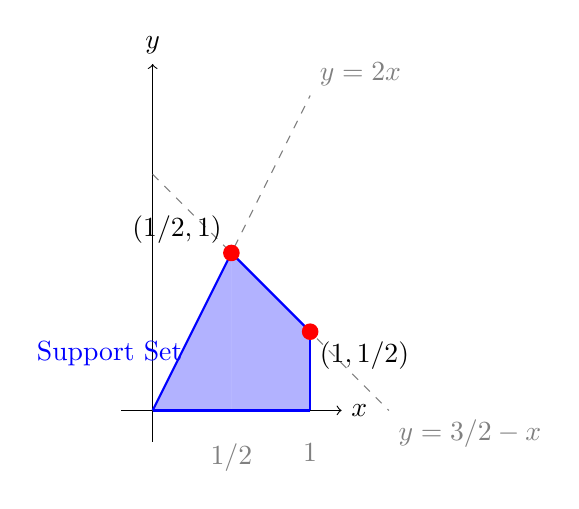
\begin{tikzpicture}[scale=2]
    % Draw axes
    \draw[->] (-0.2,0) -- (1.2,0) node[right] {$x$};
    \draw[->] (0,-0.2) -- (0,2.2) node[above] {$y$};
    
    % Draw the boundary lines
    \draw[dashed, gray] (0,0) -- (1,2) node[above right] {$y=2x$};
    \draw[dashed, gray] (0,1.5) -- (1.5,0) node[below right] {$y=3/2-x$};
    \draw[dashed, gray] (0,0) -- (1,0) node[below] {};
    
    % Fill the support region
    % Region 1: $0 < x < 1/2$, $0 < y < 2x$
    \fill[blue, opacity=0.3] (0,0) -- (0.5,0) -- (0.5,1) -- (0,0);
    
    % Region 2: $1/2 < x < 1$, $0 < y < 3/2-x$
    \fill[blue, opacity=0.3] (0.5,0) -- (1,0) -- (1,0.5) -- (0.5,1) -- (0.5,0);
    
    % Draw boundary lines more prominently
    \draw[blue, thick] (0,0) -- (0.5,1);
    \draw[blue, thick] (0.5,1) -- (1,0.5);
    \draw[blue, thick] (1,0.5) -- (1,0);
    \draw[blue, thick] (1,0) -- (0,0);
    
    % Mark special points
    \fill[red] (0.5,1) circle (1.5pt);
    \node[above left] at (0.5,1) {$(1/2, 1)$};
    
    \fill[red] (1,0.5) circle (1.5pt);
    \node[below right] at (1,0.5) {$(1, 1/2)$};
    
    % Add labels
    \node[below left, blue] at (0.25,0.5) {Support Set};
    \node[gray, below] at (0.5,-0.15) {$1/2$};
    \node[gray, below] at (1,-0.15) {$1$};
\end{tikzpicture}
\end{center}
在这个图上对联合函数积分即可.
\end{itemize}
\end{solution}
     
    
\end{example}

\section{independence of two random variables}
\subsection{independence of two random variables 的三种等价定义}
\begin{definition}{independence of random variables, def 1: joint distribution is product of marginal distributions}
    两个 random variables \(X, Y: \Omega \to \bR\) 被称为 independent 的, 
    如果对于任意的 Borel sets \(A, B \subseteq \bR\), 都有
    \[
    \bP(X \in A, Y \in B) = \bP(X \in A) \cdot \bP(Y \in B)
    \]
    注意这个定义等价于 for all points \((x, y) \in \mathbb{R}^2\),
    \[
    F_{X,Y}(x, y) = F_X(x) F_Y(y)   
    \]
    即\textbf{它们的 joint distribution 是它们 marginal distributions 的 product.}
\end{definition}
对于 discrete 和 continuous random variables 而言, 这还意味着 independence 等价于:
\begin{itemize}
        \item joint pmf 是 marginal pmfs 的 product, for discrete case.
        \item joint pdf 是 marginal pdfs 的 product, for continuous case.
\end{itemize}
详细而言: 
\begin{theorem}{discrete and continuous independence: joint density is product of marginal densities} \label{discrete and continuous case of independence: joint density is product of marginal densities}
    令 \(X, Y\) 是两个 random variables. 
    \begin{itemize}
        \item 如果 \(X, Y\) 是 discrete random variables, 
        则它们 independent 的条件等价于对于任意 \(x, y\), 都有
        \[
        p_{X,Y}(x, y) = p_X(x) \cdot p_Y(y)
        \]
        \item 如果 \(X, Y\) 是 continuous random variables, 则它们 independent 的条件等价于对于任意 \(x, y\), 都有
        \[
        f_{X,Y}(x, y) = f_X(x) \cdot f_Y(y)
        \]
    \end{itemize}
\end{theorem}
\begin{proof}
    discrete case: 显然可得.

    continuous case: 
    \begin{itemize}
        \item \(F_{X,Y}(x, y) = F_X(x) F_Y(y)  \implies f_{X,Y}(x, y) = f_X(x) \cdot f_Y(y)\): 取偏导数即可.
        \item \(f_{X,Y}(x, y) = f_X(x) \cdot f_Y(y) \implies F_{X,Y}(x, y) = F_X(x) F_Y(y)\): 积分即可.
    \end{itemize}
\end{proof}
因而对于 independent 的两个 
random variables, 固定 $X= x_0$, 那么联合密度函数
$f_{X,Y}(x_0, y)$ 就是 $Y$ 的边际密度函数 $f_Y(y)$ 乘上
一个常数 $f_X(x_0)$.\\


\begin{remark}

Recall 两个事件 independence 的定义: 
$$ 
\mathbb{P}( A \cap B) = \mathbb{P}( A) \cdot \mathbb{P}( B)
$$
也等价于对于任意的 Borel sets \(A, B\) where \(\bP(B) > 0\), 都有
$$
\mathbb{P}( A \mid B) = \mathbb{P}( A)  
$$
即: 一个事件发生与否都不会对另一个事件发生的概率产生任何影响.


而再看到两个 random variables independence 的定义是:
$$
\mathbb{P}(X \in A, Y \in B) = \mathbb{P}(X \in A) \cdot \mathbb{P}(Y \in B)
$$
这个定义也当然等价于:
\begin{proposition}{independence of random variables, def 2: conditional distribution is marginal distribution}
两个 random variables \(X, Y\) 是 independent 的, iff: 对于任意的 Borel sets \(A, B\), 
如果\(\bP(Y \in B) > 0\), 则
$$
\mathbb{P}(X \in A \mid Y \in B) = \mathbb{P}(X \in A)  
$$
即: \textbf{\(X\) 的 conditional distribution,
 不论给定 \(Y\) 的任何信息, 都等于 \(X\) 的 marginal distribution.}
\end{proposition}

所以它实际上意义是: \textbf{知道一个 random variable 的任何信息, 对于另外一个都没有任何帮助. }

因而\textbf{它们的 joint distribution 可以分解成 marginal distributions 的 product}.\\
\end{remark}

\begin{remark}

Furthermore: 我们不难发现一件事情, 可以\textbf{在 independence 
of two events 和 independence of two random variables 之间建立一个桥梁:}
\begin{proposition}{independence of random variables, 
def 3: generated sigma-algebras}
令 \(X, Y\) 是两个 random variables. 
    则 \(X, Y\) 是 independent 的 iff:
     \(X\) 生成的 sigma-algebra \(\sigma(X)\) 和 \(Y\) 生成的 sigma-algebra 
     \(\sigma(Y)\) 中分别任取一个事件, 这两个事件都是 independent 的. 即:
$$
\forall A \in \sigma(X), \forall B \in \sigma(Y), \quad 
\bP(A \cap B) = \bP(A) \cdot \bP(B)
$$
\end{proposition}
这严格说明了: \textbf{两个 random variables 之间的 independence, 
本质上是它们各自蕴含的 information
(由 generated sigma-algebra 严格刻画) 的完全不相关}:  
对 \(X\) 的观测对于
预测 \(Y\) 的任何行为都不提供任何帮助, 反之亦然.\\
\end{remark}

以上就是 independence of two random variables 的定义, 以及其 
information geometric intuition.

下面我们讲 independence between two random variables, generalize 
到 mutual independence among 任意的 family of random variables.


\subsection{mutual independence of a family of random variables: 强于 pairwise independence}
我们定义了两个 random variables 的 independence, 
但是这个定义可以推广到多个 (甚至 uncountably many) random variables 上.
\begin{definition}{\textbf{mutual independence} of multiple random variables}
    令 \(\{X_i: i \in I\}\) 是一个 random variables 的 family, 
    其中 \(I\) 是一个 index set. 
    则如果对于任意的 finite subset \(J \subseteq I\), 
    以及对于任意的 Borel sets \(\{A_j: j \in J\}\), 都有
    \[
    \bP(X_j \in A_j, \forall j \in J) = \prod_{j\in J} \bP(X_j \in A_j)
    \]
    则称这个 family of random variables 是 independent 的.
\end{definition}
注意: \textbf{joint mass $\&$ density 的 factorization 也可以推广到多个 random variables 上.} 
有一件事情值得说明: 
这里定义的是\textbf{mutual independence}, 也就是说, 对于任意的 finite subset \(J\),
它们的 joint distribution 都 factorizes into product of marginal distributions.

而\textbf{两两 independent 的 random variables family 不一定是 mutual independent 的.}
即: 如果对于任意的 \(i \neq j\), \(X_i\) 和 \(X_j\) 是 independent 的,
并不意味着对于任意的 finite subset \(J\), \(\{X_j: j \in J\}\) 是 independent 的. 

举个例子: 

\begin{example}{pairwise independence does NOT imply mutual independence}
假设我们抛掷两枚公平的硬币.
令 $X, Y$ 是两个 independent 的 random variables, 
且都服从 uniform distribution on $\{-1, 1\}$. 即:
$$
\bP(X=1) = \bP(X=-1) = \frac{1}{2}, \quad \bP(Y=1) = \bP(Y=-1) = \frac{1}{2}
$$
现在, 我们定义第三个 random variable $Z$ 为前两者的 product:
$$
Z = X \cdot Y
$$
容易验证: $X, Y, Z$ 两两 independent, 但不 mutual independent.
因为如果只是知道 $X$ 的值, 那么我们对于 $Z$ 的值完全没有信息
(因为有一个完全随机的 $Y$ 没有任何已知信息); 同样, 
如果只是知道 $Y$ 的值, 那么我们对于 $Z$ 的值也完全没有信息;

但是, 如果我们同时知道 $X$
和 $Y$ 的值, 那么 $Z$ 的值就完全确定了. 

这说明 \textbf{pairwise independence 只能保证局部的信息解耦, 
而 mutual independence 则保证了在这个 family of random variables 之间的全局信息解耦.}
\end{example}




\subsection{independent $\implies$ uncorrelated}
Independence 的概念会让我们回忆起另外一个刻画两个 random variables 
之间关系的概念: covariance, 它丈量了\textbf{两个 random variables 之间的线性关系}.

 covariance 的定义:
$$
\operatorname{Cov}(X, Y):=\mathbb{E}[(X-\mathbb{E}[X])(Y-\mathbb{E}[Y])] = \mathbb{E}[XY]-\mathbb{E}[X] \mathbb{E}[Y]
$$

我们容易发现: \textbf{independence 是一个比 covariance 为 0 (即 uncorrelated) 更强的概念:}
\begin{proposition}{independent 严格强于 uncorrelated}
    令 \(X, Y\) 是两个 random variables. 
    则 \(X, Y\) 是 independent 的 \(\implies\) \(\operatorname{Cov}(X, Y) = 0\).
    但是 \(\operatorname{Cov}(X, Y) = 0\) 不一定 \(\implies\) \(X, Y\) 是 independent 的.
\end{proposition}
\begin{proof}
\begin{itemize}
    \item independence \(\implies\) covariance 是 0, 因为 independence 显然 imply\(E[XY] = E[X]E[Y]\), 
    从而 covariance 的定义式中 \(E[XY] - E[X]E[Y] = 0\).
    \item  有一个经典反例: 考虑 \(X\) 是任意按原点对称的分布, 比如一个 standard normal distribution; 而定义 \(Y = X^2\),
此时 $$\text{Cov}(X, X^2) = E[X \cdot X^2] - E[X]E[X^2] = E[X^3] - E[X]E[X^2]$$
由于 \(X\) 的分布是关于原点对称的, \(E[X^3] = 0\) 且 \(E[X] = 0\), 因而 covariance 是 0.
但是 \(X\) 和 \(Y\) 显然不是 independent 的.
\end{itemize}
\end{proof}
\begin{remark}
本质上, independence 是一种最强的全局信息不相关性. 
而 covariance 只度量 linear relationship.  
试想: 如果这两个随机变量之间的关系是这样的呢?
\begin{center}
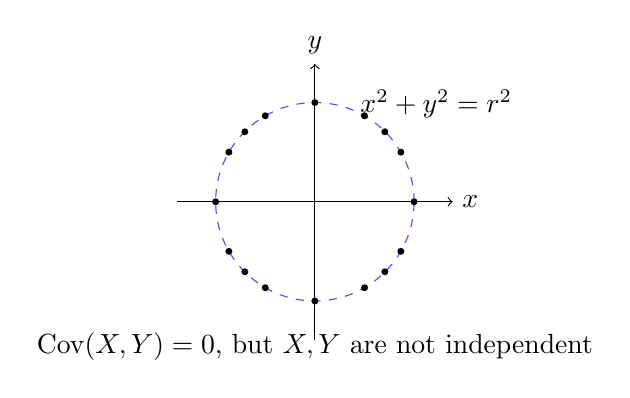
\begin{tikzpicture}[scale=0.7]
    \draw[->] (-2.5,0) -- (2.5,0) node[right] {$x$};
    \draw[->] (0,-2.5) -- (0,2.5) node[above] {$y$};
    \draw[dashed, blue!70] (0,0) circle (1.8);
    \foreach \x/\y in {
        1.8/0, 1.27/1.27, 0/1.8, -1.27/1.27,
        -1.8/0, -1.27/-1.27, 0/-1.8, 1.27/-1.27,
        1.56/0.9, 0.9/1.56, -0.9/1.56, -1.56/0.9,
        -1.56/-0.9, -0.9/-1.56, 0.9/-1.56, 1.56/-0.9
    }
        \fill (\x,\y) circle (1.8pt);
    \node[above right] at (0.65,1.35) {$x^2+y^2=r^2$};
    \node[below] at (0,-2.2) {Cov$(X,Y)=0$, but $X,Y$ are not independent};
\end{tikzpicture}
\end{center}
那么它们的 covariance 是 0, 但是它们显然不是 independent 的. 所以 covariance 
忽略了很多非线性的关系, 而 independence 则完全捕捉了所有的关系. \\
\end{remark}

刚才说到, 两个 random variables 的 independence 显然 imply 
$\mathbb{E}[XY] = \mathbb{E}[X]\mathbb{E}[Y]$.
而 BTW: 这个性质其实\textbf{可以 generalize 到任意
 finite number of independent random variables 的 product 上, 并且
 我们可以在这些 random variables 上任意地施加 Borel measurable functions}, 
 只要保证这些函数的 expectation 是 finite 的,
\begin{theorem}{independence \(\implies\) expectation is closed under product}
    令 \(\{X_i: i \in I\}\) 是一个 independent 的 random variables 的 family, 
    则对于任意的 finite subset \(J \subseteq I\), 以及对于任意的 Borel measurable functions \(\{g_j: j \in J\}\), 
    如果 \(\bE[|g_j(X_j)|] < \infty\) for all \(j \in J\), 则
    \[
    \bE\left[\prod_{j\in J} g_j(X_j)\right] = \prod_{j\in J} \bE[g_j(X_j)]
    \]
    特别地, 取每个 \(g_j(x) = x\), 则
    \[\bE\left[\prod_{j\in J} X_j\right] = \prod_{j\in J} \bE[X_j]\]
\end{theorem}
\begin{proof}
令 $J = \{1, 2, \dots, n\}$.
由于 $X_1, \dots, X_n$ 是 independent 的, 它们的 joint distribution
 $\mu_{\mathbf{X}}$ 是其 marginal distributions $\mu_{X_j}$ 的 product measure: $$\mu_{\mathbf{X}} = \mu_{X_1} \times \mu_{X_2} \times \dots \times \mu_{X_n}$$
根据 Change of Variables Formula, 
$$\bE\left[\prod_{j=1}^n g_j(X_j)\right] = \int_{\bR^n} 
\left( \prod_{j=1}^n g_j(x_j) \right) \, d\mu_{\mathbf{X}}(x_1, \dots, x_n)
= \int_{\bR} \dots \int_{\bR} \left( \prod_{j=1}^n g_j(x_j) \right) \, d\mu_{X_1}(x_1) \dots d\mu_{X_n}(x_n)
$$
由于被积函数 $\prod g_j(x_j)$ 是变量分离的, 根据 Fubini's Theorem 可以把积分分解成多个积分的 product:
$$= \left( \int_{\bR} g_1(x_1) \, d\mu_{X_1}(x_1) \right) \times \dots \times \left( \int_{\bR} g_n(x_n) \, d\mu_{X_n}(x_n) \right)$$
其中每一项都是$\bE[g_j(X_j)]$.
\end{proof}
\begin{remark}
recall: expectation is a linear operator (因而 linearity 是 regardless of independence).
但是它不一定是一个 multiplicative operator. 

而这里我们说, \textbf{如果 random variables 是 independent 的, 那么 expectation 就是一个 multiplicative operator.}
\end{remark}


实际上: 当这些 Borel measurable functions \(\{g_j: j \in J\}\) 
全都 bounded 时, 这个定理其实反向也是成立的:
\begin{theorem}
    令 \(\{X_i: i \in I\}\) 是一个family of random variables.
    如果对于任意的 finite subset \(J \subseteq I\), 以及任意的
     bounded Borel measurable functions \(\{g_j: j \in J\}\), 都有
    \[
    \bE\left[\prod_{j\in J} g_j(X_j)\right] = \prod_{j\in J} \bE[g_j(X_j)]
    \]
    则这个 family of random variables 是 independent 的.
\end{theorem}
\begin{proof}
不妨特取 indicator functions.
对于任意的 Borel sets $A, B \subseteq \bR$, 
令 $f(x) = I_A(x)$, $g(y) = I_B(y)$.
代入等式得到:$$\bE[I_A(X) \cdot I_B(Y)] = \bE[I_A(X)] \cdot \bE[I_B(Y)]$$
注意到 $I_A(X) \cdot I_B(Y) = I_{\{X \in A, Y \in B\}}$. 根
据 expectation of indicator function 等于 probability,
我们立刻得到:$$\bP(X \in A, Y \in B) = \bP(X \in A) \cdot \bP(Y \in B)$$
\end{proof}
注意:\textbf{ \(g(x) = x\) 并不是 bounded 的 function, 因而 uncorrelation $\not \implies$ independence.}\\


OK. 以上是 pretty much general properties of independence. 
最后我们看一下, 对于 discrete 和 continuous random variables 而言, 
independence 的 characterization 具体长什么样子.






\subsection{discrete RV independence 的 characterization}
\begin{remark}
关于两个 discrete random variables \(X, Y\) 是否 independent 的判断,
还有一个直观的方法.
\begin{proposition}{discrete RV independence 的 characterization}\label{discrete RV independence 的 characterization}
    两个 discrete random variables \(X, Y\) 
    是 independent 的 iff 它们的 joint pmf as a matrix 
    有 rank 1(每行每列都互为倍数).
\end{proposition}
\begin{proof}
note: 一个矩阵 $M$ 的 rank 等于 1 iff 它可以被分解为两个向量的 outer product
:$$M = \mathbf{u}\mathbf{v}^\top$$\
where $\mathbf{u}$ 和 $\mathbf{v}$ 是非零列向量.

($\implies$): 如果 independent, 
那么对于所有 $i, j$,
joint probability $p_{ij} = \bP(X=x_i, Y=y_j)$ 
满足:$$p_{ij} = \bP(X=x_i) \cdot \bP(Y=y_j)$$
如果我们定义向量 $\mathbf{p}_X = [p_X(x_1), p_X(x_2), \dots]^\top$ 
和 $\mathbf{p}_Y = [p_Y(y_1), p_Y(y_2), \dots]^\top$, 
那么整个联合分布矩阵 $P$ 就可以写成:$$P = \mathbf{p}_X \mathbf{p}_Y^\top$$
这正是 Rank 1 矩阵的标准形式. 

($\impliedby$) 
如果 $P$ 的 rank 为 1, 
那么存在向量 $\mathbf{u}$ 和 $\mathbf{v}$ 
使得 $p_{ij} = u_i v_j$.由于 $\sum_{i,j} p_{ij} = 1$, 
我们可以归一化这两个向量, 使得 $\sum u_i = 1$ 
且 $\sum v_j = 1$.此时, $u_i$ 恰好就是 $X$ 的 marginal PMF, 
$v_j$ 恰好就是 $Y$ 的 marginal PMF. 因此满足 $p_{ij} = p_i \cdot p_j$, 即两个变量独立.
\end{proof}
\begin{example}
    \[
    P = 
    \begin{array}{c|cc|c}
    X \backslash Y & 0 & 1 & \text{Marginal } \bP(X) \\ \hline
    0 & 0.4 & 0.1 & 0.5 \\
    1 & 0.4 & 0.1 & 0.5 \\ \hline
    \text{Marginal } \bP(Y) & 0.8 & 0.2 & 1.0
    \end{array}
    \]
这里的 \(X,Y\) 就是 independent 的 random variables.
\end{example}
\end{remark}

\subsection{continuous RV independence 的 geometric intuition}
对于 independent continuous random variables \(X, Y\), 它的 characterization 
我们已经知道了: 即 joint pdf factorizes into marginal pdfs. 
这一个 characterization 的 geometric intuition 是:  
\begin{itemize}
    \item joint pdf 的 support set 一定是一个矩形 (不一定 bounded)
    \item joint pdf 的\textbf{每个维度上的任意截面的形状都是一样的} (因为固定 \(x\), 则 \(y\) 方向的性质只由 \(f_Y\) 决定.)

即: 固定 \(x\), \(y\)-distribution 的横截面永远长得像 \(f_Y\), 只是乘上了一个常数 \(f_X(x)\) 而已. 同样的, 固定 \(y\), \(x\) 分布的横截面永远长得像 \(f_X\), 只是乘上了一个常数 \(f_Y(y)\) 而已.
\end{itemize}

\begin{center}
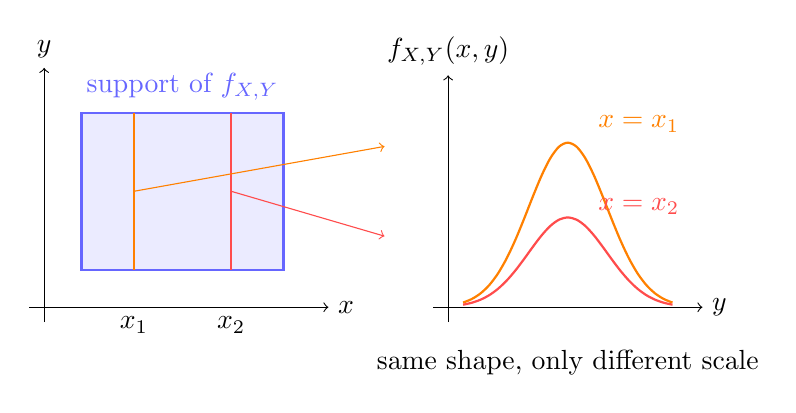
\begin{tikzpicture}[scale=0.95]
    \begin{scope}
        \draw[->] (-0.2,0) -- (3.8,0) node[right] {$x$};
        \draw[->] (0,-0.2) -- (0,3.2) node[above] {$y$};
        \fill[blue!8] (0.5,0.5) rectangle (3.2,2.6);
        \draw[thick, blue!60] (0.5,0.5) rectangle (3.2,2.6);
        \draw[thick, orange] (1.2,0.5) -- (1.2,2.6);
        \draw[thick, red!70] (2.5,0.5) -- (2.5,2.6);
        \node[below] at (1.2,0) {$x_1$};
        \node[below] at (2.5,0) {$x_2$};
        \node[blue!60] at (1.85,2.95) {support of $f_{X,Y}$};
        \draw[->, orange] (1.2,1.55) -- (4.55,2.15);
        \draw[->, red!70] (2.5,1.55) -- (4.55,0.95);
    \end{scope}

    \begin{scope}[xshift=5.4cm]
        \draw[->] (-0.2,0) -- (3.4,0) node[right] {$y$};
        \draw[->] (0,-0.2) -- (0,3.1) node[above] {$f_{X,Y}(x,y)$};
        \draw[thick, orange, domain=0.2:3.0, smooth] plot (\x,{2.2*exp(-((\x-1.6)^2)/0.55)});
        \draw[thick, red!70, domain=0.2:3.0, smooth] plot (\x,{1.2*exp(-((\x-1.6)^2)/0.55)});
        \node[orange] at (2.55,2.45) {$x=x_1$};
        \node[red!70] at (2.55,1.35) {$x=x_2$};
        \node[below] at (1.6,-0.45) {same shape, only different scale};
    \end{scope}
\end{tikzpicture}
\end{center}





\section{conditional distribution function and density}
\subsection{conditional distribution and its distribution function}
\begin{definition}{conditional distribution}
给定 random variables \(X, Y: \Omega \to \mathbb{R}\), 
我们定义 the conditional distribution of \(X\) given \(Y = y\) 
为 the probability measure \(\bP^{X|Y=y}\):
\[
\bP^{X|Y=y}(A) := \lim_{h\to 0^+} \bP(X \in A \mid y \leq Y \leq y+h),\quad \forall A \in \cB(\bR)
\]
并将 function \(F_{X|Y=y}: \bR \to \bR\) defined by \(F_{X|Y=y}(x) := \bP^{X|Y=y}((-\infty, x])\):
\[
F_{X|Y}(x|y) := \lim_{h\to 0^+} \bP(X\leq x \mid y \leq Y \leq y+h)
\]
称为 the conditional distribution function of \(X\) given \(Y=y\).
\end{definition}
\begin{remark}
注意: 每个取值 \(y\) 都对应一个 conditional distribution measure \(\bP^{X|Y=y}\) 
和一个 conditional distribution function \(F_{X|Y=y}\).
因此, conditional distribution 和 conditional distribution function 都是一个 family of measures/functions,
而不是一个 measure/function.

也就是说, 一个 random variable 可以 induce 出另一个 random variable 的可能 uncountably many 个 conditional distribution.
\end{remark}

\begin{remark}
    如果 \(X,Y\) 是两个 discrete random variables, 那么它们的 conditional distribution 就很简单了.
    \[
    \bP^{X|Y=y}(\{x\}) = \frac{\bP(X=x, Y=y)}{\bP(Y=y)}
    \]
    以及
    \[
    F_{X|Y=y}(x) = \sum_{t\leq x} \frac{\bP(X=t, Y=y)}{\bP(Y=y)}
    \]

    其他情况稍复杂一些. 但是我们可以确定的是:
\end{remark}

\subsection{conditional density for random variables jointly continuous}
\begin{theorem}{jointly continuous RVs 之间所有 defined 处总有 conditional density}\label{jointly continuous random variables 之间总有 conditional density}
    令 \(\mathbf{X} = (X, Y)^T\) 是一个 continuous random vector, 
    则对于任意 \(y\) 使得 \(f_Y(y) > 0\), 都有 conditional distribution of \(X\) given \(Y=y\) 的 pdf:
    \[
    f_{X|Y}(x|y) := \frac{f_{X,Y}(x,y)}{f_Y(y)}
    \]
    即: \(\forall x \in \bR\) 有: \[
    F_{X |Y}(x|y) = \int_{-\infty}^x \frac{f_{X,Y}(t,y)}{f_Y(y)} \, dt
    \]
\end{theorem}
\begin{proof}
注意: \((X,Y)^T\) 是 continuous random vector \(\implies\) \(Y\) 是一个 continuous random variable. 因而
因而 \(f_Y(y)\) 是 well-defined 的. (反过来不成立)
取 \(y\) s.t. \(f_Y(y) > 0\).

则 
\begin{align*}
    \mathbb{P}^{X \mid Y=y}(A) &=\lim _{h \rightarrow 0^{+}} \mathbb{P}(X \in A \mid y \leq Y \leq y+h) \\
    &= \lim _{h \rightarrow 0^{+}} \frac{\mathbb{P}(X \leq x, y \leq Y \leq y+h)}{\mathbb{P}(y \leq Y \leq y+h)}=\lim _{h \rightarrow 0^{+}} \frac{F_{X, Y}(x, y+h)-F_{X, Y}(x, y)}{F_Y(y+h)-F_Y(y)}\\
    &=\frac{\partial_y F_{X, Y}(x, y)}{f_Y(y)}=\int_{-\infty}^x \frac{f_{X, Y}(s, y)}{f_Y(y)} ds
\end{align*}
因而, \(f_{X|Y}(x|y) := \frac{f_{X,Y}(x,y)}{f_Y(y)}\) 是 \(F_{X|Y=y}\) 的 pdf.
\end{proof}
\begin{remark}
    为了保证 continuous random vector 下分量之间的 conditional distribution 总是 (a.e.) 拥有 pdf 的, 我们可以
    给 not well-defined 处下定义: 如果 \(f_Y(y) = 0\), 就直接 set \(f_{X|Y}(x|y) = 0\) for all \(x\).
    
    在这个定义下: continuous random vector 下分量之间的 conditional distribution 也总是 continuous 的.
\end{remark}


\subsection{Law of Total Probability for continuous random vector}
\begin{theorem}\label{law of total probability for continuous random vector}
    令 \(\mathbf{X} = (X, Y)^T\) 是一个 continuous random vector, 
    则对于任意 \(A \in \mathcal{B}(\bR) \), 
    \[
    \mathbb{P}((X, Y) \in A)=\int_{-\infty}^{+\infty} \mathbb{P}((X, y) \in A \mid Y=y) f_Y(y) d y
    \]
\end{theorem}
\begin{proof}
    注意: \[
    \mathbb{P}\left(Y \in\left\{y \in \mathbb{R}: f_Y(y)=0\right\}\right)=0
    \]
    即, \(\left\{Y \in f_Y^{-1}(\{0\})\right\} \) 是一个 null set. (不是说 \(f_Y(y) = 0\) 的 \(y\) 是 null set, 
    意思是说 \(Y\) 落在这些 \(y\) 上的事件是 null set.)

    因而 compute: 
    \begin{align*}
\mathbb{P}(X \in(-\infty, x], Y \leq y) & =\mathbb{P}\left(X \in(-\infty, x],\{Y \leq y\} \cap\left\{Y \notin f_Y^{-1}(\{0\})\right\}\right)=\int_{(-\infty, y] \cap f_Y^{-1}\left(\{0\}^c\right)} \int_{-\infty}^{\infty} f_{X, Y}(s, t) d s d t \\
& =\int_{(-\infty, y] \cap f_Y^{-1}((0,+\infty))}\left(\int_{-\infty}^x \frac{f_{X, Y}(s, t)}{f_Y(t)} d s\right) f_Y(t) d t \\
& =\int_{(-\infty, y] \cap f_Y^{-1}((0,+\infty))} \mathbb{P}(X \leq x \mid Y=t) f_Y(t) d t \\
& =\int_{(-\infty, y] \cap f_Y^{-1}((0,+\infty))} \mathbb{P}(X \leq x \mid Y=t) f_Y(t) d t+\int_{(-\infty, y] \cap f_Y^{-1}(\{0\})} \mathbb{P}(X \leq x \mid Y=t) f_Y \\
& =\int_{(-\infty, y]} \mathbb{P}(X \leq x \mid Y=t) f_Y(t) d t \\
& =\int_{-\infty}^y \mathbb{P}(X \leq x \mid Y=t) f_Y(t) d t
\end{align*}
\end{proof}
\begin{remark}
    recall 最普通的全概率公式: 把样本空间 partition 成几个 disjoint 的事件 \(B_1, \cdots, B_n\),
    则任意事件\(A\) 等于它在每个 \(B_i\) 上的 conditional probability 的和:
    $$\mathbb{P}(A) = \sum_{i=1}^n \mathbb{P}(A \cap B_i) = \sum_{i=1}^n \mathbb{P}(A \mid B_i) \mathbb{P}(B_i)$$
    这很容易理解. 而这里的 law of total probability for continuous random vector 就是这个公式在 continuous case 的推广:

    由于在每一点 \(y\) 上, \((X,Y) \in A\) 的概率都有一个 conditional distribution \((X,Y)\in A | Y = y\), 因而
    \((X,Y) \in A\) 的概率就等于这个 conditional distribution 在所有 \(y\) 上的加权和, 权重就是 \(Y\) 的 pdf \(f_Y(y)\). 
    因而才有 \[
    \mathbb{P}((X, Y) \in A)=\int_{-\infty}^{+\infty} \mathbb{P}((X, y) \in A \mid Y=y) f_Y(y) d y
    \]
\end{remark}

\begin{example}
考虑 random vector \(\mathbf{X} = (X, Y)^T\) with joint pdf
\[
f_{X, Y}(x, y)= \begin{cases}4 x y, & \text { if } 0 \leq x \leq 1,0 \leq y \leq 1 \\ 0, & \text { otherwise }\end{cases}
\]
计算: \(f_X, f_Y, f_{X|Y}, f_{Y|X}\).

\begin{solution}
首先计算 margianl pdfs:
\[
f_X(x)=\int_{-\infty}^{+\infty} f_{X, Y}(x, y) d y=\int_0^1 4 x y d y=2 x, \text { for } 0 \leq x \leq 1
\]
and
\[
f_Y(y)=\int_{-\infty}^{+\infty} f_{X, Y}(x, y) d x=\int_0^1 4 x y d x=2 y, \text { for } 0 \leq y \leq 1
\]
由于这是一个 continuous random vector, 因而根据\ref{jointly continuous random variables 之间总有 conditional density} 可以得到:
\[
f_{X \mid Y}(x \mid y)= \begin{cases}\frac{f_{X, Y}(x, y)}{f_Y(y)}=\frac{4 x y}{2 y}=2 x, & \text { if } x \in[0,1], \\ 0, & \text { otherwise. }\end{cases}
\]
同理计算出
\[
f_{Y \mid X}(y \mid x)= \begin{cases}\frac{f_{X, Y}(x, y)}{f_X(x)}=\frac{4 x y}{2 x}=2 y, & \text { if } y \in[0,1], \\ 0, & \text { otherwise. }\end{cases}
\]
\end{solution}
\end{example}




\section{conditional expectation}
\begin{definition}{conditional expectation}\label{conditional expectation}
令 \(X, Y: \Omega \to \mathbb{R}\) 为 RVs. 
对于 \(y \in \mathbb{R}\) where \(F_{X|Y} = \bP^{X|Y =y}(X\leq x)\) is defined
 (这个条件对于 discrete 是筛选掉 \(\bP(y) =0\) 的点, 对于 continuous 这是为了筛选掉 \(f_Y = 0\) 的点), 
 我们定义 conditional expectation:
  \[
  \bE[X | Y = y] := \int_{-\infty}^{\infty} x \, d\bP^{X|Y=y}(x) 
  \]
  特别地, 如果\((X,Y)\) 是一个 discrete random vector, 则它即是:
  \[
   \bE[X | Y = y] = \sum_{x} x \bP(X | Y)(x|y) = \sum_{x} x \bP(X = x | Y = y)
  \]
  而如果 \((X,Y)\) 是一个 (absolutely) continuous random vector, 则它即是:
  \[
   \bE[X | Y = y] = \int_{-\infty}^{\infty} x f_{X|Y}(x|y) \, dx
  \]
\end{definition}
\begin{remark}
    注意: conditional expectation 对于给定的 \(y\) 是一个值;
     而它也整体是一个 function of \(y\), 同时也是 function from the sample space \(\Omega\)
 (更准确而言是 \(\{ \omega \in \Omega : f_Y(Y(\omega))>0  \}\), 但是去掉的
 这个集合的测度为零, 所以不用管, a.e. define 即可).

     对于 \(\omega \in \Omega\), \[
     \bE[X|Y]: \omega \mapsto \bE[X|Y=Y(\omega)]
     \]
     Notice: 这个函数是一个 random variable.
    同理, 我们可以构造 conditional expectation 
    given multiple random variables \(\bE[X|Y_1, \cdots, Y_n]\). 但是暂时不谈论这个.
\end{remark}


\begin{proposition}{independence 让 conditional distribution, density 和 expectation 都退化}
    如果 \(X,Y\) 是 independent 的, 那么在任意 defined \(y\) 上, 
    \[
    F_{X|Y=y} = F_X, \quad f_{X|Y=y} = f_X, 
    \]
    以及 \[
    \quad \bE[X|Y] = \bE[X]
    \]
\end{proposition}


\begin{example}\textbf{(constant random variable 的 conditional expectation)}

令 \(X :=b\) 为一个 constant random variable. 
\(Y\) 为一个 (absolutely) continuous random variable.
compute: \(\bE[X|Y]\) when \(f_Y(y) > 0\).

\begin{solution}
    \[
    F_{X, Y}(x, y)=\mathbb{P}(X \leq x, Y \leq y)=\left\{\begin{array}{ll}
F_Y(y), & \text { if } x \leq b, \\
0, & \text { if } x>b
\end{array}=F_X(x) \cdot F_Y(y)\right.
\]
因而它们 independent (当然,,)
因而 \[
\bE[X|Y] = \bE[X] = b
\]
\end{solution}
为什么我们要提及这个很呆的例子
因为我们要说一个很呆但是要说一下的事情: 
\begin{proposition}
conditional expectation 满足 linear property.
即任取 \(a,b\in\bR\), \[
\bE[aX + b|Y] = a\bE[X|Y] + b
\]
\end{proposition} 
\end{example}

\begin{example}
    (computation exercise)
    令 \(X,Y\) 为 RVs with joint pdf \[
    f_{X, Y}(x, y)= \begin{cases}\frac{1}{y} e^{-\frac{x}{y}} e^{-y}, & x>0, y>0 \\ 0, & \text{otherwise}\end{cases}
    \]
    计算: \(\bE[X|Y=y]\).

    \begin{solution}
        根据 \ref{jointly continuous random variables 之间总有 conditional density} 和 
        \ref{conditional expectation}, 我们就是要做两件事情: 一个是计算 \(f_Y\), 然后
        根据 \(f_Y\) 和 \(f_{X,Y}\) 计算出 \(f_{X|Y}\), 
        最后根据 \(f_{X|Y}\) 积分计算出 \(\bE[X|Y]\).

        那么 \[
        f_Y(y)=\int_{-\infty}^{+\infty} f_{X, Y}(x, y) d x=e^{-y} \int_0^{+\infty} \frac{1}{y} e^{-x / y} d x=e^{-y}, y>0
        \]
        我们发现 \(Y \sim \text{Exp}(1)\). 然后对于 \(y>0\), \[
        f_{X \mid Y}(x \mid y)=\frac{f_{X, Y}(x, y)}{f_Y(y)}=\frac{1}{y} e^{-x / y}
        \]
        因而 \(X|Y = y \sim \text{Exp}(1/y)\).
        最后, \[
        \mathbb{E}[X \mid Y=y]=\int_{-\infty}^{+\infty} x f_{X \mid Y}(x \mid y) d x=\frac{1}{y} \int_0^{+\infty} x e^{-x / y} d x=y
        \]
        而对于 \(y \leq 0\), 因为 \(f_Y(y) = 0\), $\mathbb{E}[X \mid Y=y]$ is not defined.
    \end{solution}
\end{example}


//TODO: 如果 \(X\) 是 continous 的, 而 \(Y\) 是 discrete 的,
那么我们怎么 define conditional distribution, 以及 expectation 呢?
这个时候我们就需要用到
之前说的 generated \(\sigma\)-algebra 的概念了.








\section{law of total expectation}
\begin{theorem}{law of total expectation}
    令 \(X, Y: \Omega \to \bR \) 为 RVs, 我们知道它们的 conditional expectation \(\bE[X|Y]\) 也是一个 \(\Omega \to \bR\) 的 RV.

    如果 \(\bE[|\bE[X|Y]|] < \infty\), 则
    \[
    \bE[X] = \bE[\bE[X|Y]]
    \]
\end{theorem}
\begin{proof}
对于更加严格的 conditional expectation 的定义而言
 (as an orthogonal projection from \(L^2(\Omega, \mathcal{F}, \mathbb{P})\) 
 onto the subspace of \(Y\)-measurable functions), 这个定理是 trivial 的, 直接 follow from def. 
在该定义中, \(\bE[X|Y]\) 被定义为一个 \(\sigma(Y)\)-measurable function \(Z\), 
使得对于任意 \(A \in \sigma(Y)\), 都有 \[
\int_A Z \, d\mathbb{P} = \int_A X \, d\mathbb{P}
\]
那么取 \(A = \Omega\), 自然得到.

而我们目前的定义下, 要证明它则要对于 discrete 和 continuous 两种情况分别计算证明.
(recall Lebesgue Decomposition Theorem: 
任意 measure 都可以被分解成一个 discrete 的部分和一个 continuous 的部分以及一个
可以忽略的 singular 的部分. 因而证明了 discrete 和 continuous 两种情况即可.)

For discrete case:
\begin{align*}
\mathbb{E}[\mathbb{E}[X \mid Y]] & =\mathbb{E}_\omega[\mathbb{E}[X \mid Y=Y(\omega)]]=\mathbb{E}_\omega\left[\sum_x x \mathbb{P}(X=x \mid Y=Y(\omega))\right] \\
& =\sum_x x \mathbb{E}_\omega[\mathbb{P}(X=x \mid Y=Y(\omega))] \\
& =\sum_x x \sum_y \mathbb{P}(X=x \mid Y=y) \cdot \mathbb{P}(Y=y) \\
& =\sum_x x \sum_y \mathbb{P}(X=x, Y=y) \\
& =\sum_x x \mathbb{P}(X=x)=\mathbb{E}[X]
\end{align*}

For continuous case:
\begin{align*}
\mathbb{E}[\mathbb{E}[X \mid Y]] & =\mathbb{E}_\omega\left[\int_{-\infty}^{+\infty} x f_{X \mid Y}(x \mid Y(\omega)) d x\right]=\int_{-\infty}^{+\infty} x \mathbb{E}_\omega\left[f_{X \mid Y}(x \mid Y(\omega))\right] d x \\
& =\int_{-\infty}^{+\infty} x \int_{-\infty}^{+\infty} f_{X \mid Y}(x \mid y) f_Y(y) d y d x \\
& =\int_{-\infty}^{+\infty} \int_{-\infty}^{+\infty} x f_{X, Y}(x, y) d x d y \\
& =\int_{-\infty}^{+\infty} x \int_{-\infty}^{+\infty} f_{X, Y}(x, y) d x d x \\
& =\int_{-\infty}^{+\infty} x f_X(x) d x=\mathbb{E}[X]
\end{align*}
\end{proof}



\begin{example}
    (\textbf{fair coin toss})
我们投掷一枚 fair coin.
\(X_1\): 直到 HH 出现钱, 投掷的次数;

\(X_2\): 直到 HT 出现钱, 投掷的次数.

问题: 计算 \(\bE[X_1]\) 和 \(\bE[X_2]\).

\begin{solution}
    We condition on 第一次 toss \(Y_1\), 以及第二次 toss \(Y_2\).


\begin{align*}
\mathbb{E}\left[X_1\right] & =\mathbb{E}\left[\mathbb{E}\left[X_1 \mid Y_1\right]\right]=\frac{1}{2} \mathbb{E}\left[X_1 \mid Y_1=H\right]+\frac{1}{2} \mathbb{E}\left[X_1 \mid Y_1=T\right] \\
& =\frac{1}{2}\left(\frac{1}{2} \mathbb{E}\left[X \mid Y_1=H, Y_2=H\right]+\frac{1}{2} \mathbb{E}\left[X \mid Y_1=H, Y_2=T\right]\right)+\frac{1}{2}\left(1+\mathbb{E}\left[X_1\right]\right) \\
& =\frac{1}{2}\left(\frac{2}{2}+\frac{1}{2}\left(\mathbb{E}\left[X_1\right]+2\right)\right)+\frac{1}{2}\left(1+\mathbb{E}\left[X_1\right]\right) .
\end{align*}
解出 \(\bE[X_1] = 6\).
同理, 可以解出 \(\bE[X_2] = 4\).
\end{solution}

\end{example}



\begin{example}
一只鸡在一段时间内下 \(N\) 个蛋, 其中 \(N \sim \text{Pois}(\lambda)\).
每只蛋孵化成小鸡的概率为 \(p\), 互相独立.
令 \(K\) 表示孵化成小鸡的蛋的数量, 计算 \(K|N, \bE[K]\), 以及 
\(K\) 的 distribution.
\begin{solution}
由题意得 \[
\bP(K=k | N=n) = \binom{n}{k} p^k (1-p)^{n-k}
\]
因此, \(K|N =n \sim \text{Bin}(n,p)\) 因而 \(\bE[K|N=n] = np\).
由 law of total expectation, 
\[
\bE[K] = \bE[\bE[K|N]] = \bE[N] \cdot p = \lambda 
\]
然后由 law of total probability,
\begin{align*}
\bP(K=k) &= \sum_{n=k}^{+\infty} \bP(K=k, N=n) 
= \sum_{n=k}^{+\infty} \bP(K=k | N=n) \cdot \bP(N=n) \\
&= \sum_{n=k}^{+\infty} \binom{n}{k} p^k (1-p)^{n-k} \cdot \frac{\lambda^n e^{-\lambda}}{n!} \\
&= \sum_{n=k}^{+\infty} \frac{n!}{k!(n-k)!} p^k (1-p)^{n-k} \cdot \frac{\lambda^n e^{-\lambda}}{n!} \\
&= \sum_{n=k}^{+\infty} \frac{\lambda^n e^{-\lambda}}{k!(n-k)!} p^k (1-p)^{n-k} \\
&= \sum_{n=k}^{+\infty} \frac{(\lambda p)^k (\lambda (1-p))^{n-k} e^{-\lambda}}{k!(n-k)!} \\
&= \frac{(\lambda p)^k e^{-\lambda}}{k!} \sum_{n=k}^{+\infty} \frac{(\lambda (1-p))^{n-k}}{(n-k)!} \\
&= \frac{(\lambda p)^k e^{-\lambda}}{k!} \sum_{m=0}^{+\infty} \frac{(\lambda (1-p))^m}{m!} \\
&= \frac{(\lambda p)^k e^{-\lambda}}{k!} \cdot e^{\lambda (1-p)} = \frac{(\lambda p)^k e^{-\lambda p}}{k!}
\end{align*}
因而 \(K \sim \text{Pois}(\lambda p)\).
\end{solution}
\end{example}


\begin{example}
令 \((X,Y)\) 为一对 continuous RVs with joint pdf:
\[
f_{X,Y}(x,y) = 2e^{-(x+2y)} \mathbf{1}_{ \{x>0, y>0\}}
\]
首先, verify \(f_{X,Y}\) is a valid joint pdf, 然后计算 
\(\bE[X|Y=y]\) 和 \(\bE[X]\).
\begin{solution}
\[
\int_0^{\infty} \int_0^{\infty} 2 e^{-(x+2 y)} d x d y=\int_0^{\infty} 2 e^{-2 y}\left(\int_0^{\infty} e^{-x} d x\right) d y=\int_0^{\infty} 2 e^{-2 y} d y=1
\]
verify 很简单. 然后我们首先计算 density of \(Y\):
\[
f_Y(y)=\int_0^{\infty} 2 e^{-(x+2 y)} d x=2 e^{-2 y}, \quad y>0
\]
然后计算 conditional density of \(X\) given \(Y=y\):
\[
f_{X \mid Y}(x \mid y)=\frac{f_{X, Y}(x, y)}{f_Y(y)}=e^{-x}, \quad x>0
\]
因而 by \ref{conditional expectation}, \[
\bE[X \mid Y=y]=\int_0^{\infty} x e^{-x} d x=1
\]
然后 by law of total expectation, \[
\bE[X] = \bE[\bE[X|Y]] = \bE[1] = 1
\] since \(\bE[X|Y]\) is a constant function.
\end{solution}
\end{example}